\documentclass{standalone}
\usepackage{tikz}
\usepackage{ctex,siunitx}
\setCJKmainfont{Noto Serif CJK SC}
\usepackage{tkz-euclide}
\usepackage{amsmath}
\usetikzlibrary{patterns, calc}
\usetikzlibrary {decorations.pathmorphing, decorations.pathreplacing, decorations.shapes,}

\begin{document}
\small
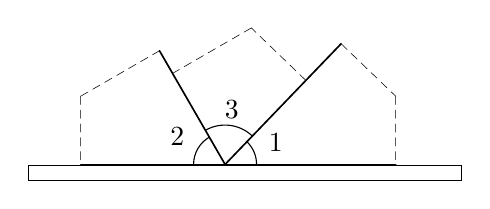
\begin{tikzpicture}[>=stealth,scale=1]
  \tkzSetUpPoint[fill=black]
  % \useasboundingbox(-1,-0.75)rectangle(3.7,1.4);
  \tkzDefPoints{0/0/B, 4/0/C, 2.5/2.6/A}
  \tkzDefTriangleCenter[centroid](A,B,C) \tkzGetPoint{G}
  \tkzDefPointBy[projection = onto  B--C](G) \tkzGetPoint{D}
  \tkzDefPointBy[projection = onto  B--A](G) \tkzGetPoint{F}
  \tkzDefPointBy[projection = onto  A--C](G) \tkzGetPoint{E}
  \tkzDefPointsBy[translation = from C to B](C,D,G,E){C1,D1,G1,E1}
  \tkzDefMidPoint(A,B)\tkzGetPoint{M}
  \tkzDefPointsBy[rotation = center M angle 180](A,F,G,E){A1,F2,G2,E2}
  \tkzDrawSegments[densely dashed](G1,D1 G1,E1 F,G G,D G2,E2 F2,G2)
  \tkzDrawSegments[semithick](D1,B B,E1 F,B B,D)
  \tkzMarkAngle[size=0.5](A,B,E1)
  \tkzLabelAngle[pos=0.7](A,B,E1){3}
  \tkzMarkAngle[size=0.4](C,B,A)
  \tkzLabelAngle[pos=0.7](C,B,A){1}
  \tkzMarkAngle[size=0.4](E1,B,D1)
  \tkzLabelAngle[pos=0.7](E1,B,D1){2}
  \draw(-2.5,-0.01)rectangle(3,-0.2);
\end{tikzpicture}
\end{document}